% !TeX program = xelatex
\documentclass[UTF8,fontset=fandol,10pt,a4paper]{ctexart}
\usepackage[left=22mm,right=22mm,top=23mm,bottom=22mm,headheight=14pt]{geometry}
\usepackage{fontspec}
\setmainfont{TeX Gyre Heros}
\setsansfont{TeX Gyre Heros}
\setmonofont{Latin Modern Mono}
\renewcommand{\familydefault}{\sfdefault}
\usepackage[table]{xcolor}
\usepackage{graphicx,tikz}
\usetikzlibrary{arrows.meta,positioning,fit,backgrounds,calc}
\usepackage{booktabs,tabularx,array,enumitem,float,caption,fancyhdr,hyperref}
\definecolor{blue}{HTML}{2869A9}
\definecolor{ink}{HTML}{293340}
\definecolor{muted}{HTML}{647181}
\definecolor{line}{HTML}{C5D4E2}
\definecolor{pale}{HTML}{F0F5FA}
\definecolor{warm}{HTML}{FFF7E9}
\hypersetup{colorlinks=true,urlcolor=blue,linkcolor=blue,pdftitle={Redflag RHI 与 Vulkan 接入设计},pdfauthor={Redflag}}
\color{ink}
\setlength{\parindent}{0pt}
\setlength{\parskip}{6pt}
\linespread{1.16}
\setlist[itemize]{leftmargin=1.5em,itemsep=2pt,topsep=3pt}
\setlist[enumerate]{leftmargin=1.8em,itemsep=3pt,topsep=3pt}
\renewcommand{\arraystretch}{1.38}
\newcolumntype{Y}{>{\raggedright\arraybackslash}X}
\newcolumntype{L}[1]{>{\raggedright\arraybackslash}p{#1}}
\ctexset{section={format=\Large\bfseries\color{blue},beforeskip=16pt,afterskip=8pt},subsection={format=\large\bfseries\color{blue},beforeskip=11pt,afterskip=5pt}}
\captionsetup{font=small,labelfont=bf,textfont={color=muted},skip=7pt}
\pagestyle{fancy}\fancyhf{}
\fancyhead[L]{\small\color{muted}Redflag · RHI / Vulkan · 设计方案}
\fancyhead[R]{\small\color{muted}2026-11-21}
\fancyfoot[C]{\small\color{muted}\thepage}
\renewcommand{\headrulewidth}{0pt}
\newcommand{\note}[1]{{\small\color{muted}#1\par}}
\newcommand{\code}[1]{{\small\texttt{#1}}}
\newcommand{\ruleline}{\par\vspace{4pt}{\color{line}\hrule}\vspace{8pt}}
\newcommand{\source}[2]{{\small\href{#1}{[#2]}}}
\tikzset{
 module/.style={draw=line,fill=pale,rounded corners=2pt,align=center,inner sep=7pt,text width=3.8cm,minimum height=1.15cm,font=\small},
 smallbox/.style={module,text width=2.55cm,minimum height=.95cm,font=\footnotesize},
 wide/.style={module,text width=9.5cm},
 planned/.style={module,fill=warm,dashed},
 flow/.style={-{Stealth[length=2mm]},draw=muted,line width=.65pt},
 own/.style={flow,dashed},
 label/.style={font=\scriptsize,fill=white,inner sep=2pt,text=muted}}

\hypersetup{pdftitle={Redflag 技术选型与工程取舍}}
\fancyhead[L]{\small\color{muted}Redflag · 技术选型与取舍}
\fancyhead[R]{\small\color{muted}2026-11-22}
\newcommand{\loc}[1]{\par{\footnotesize\color{muted}源码见 \path{#1}。}\par}
\renewcommand{\note}[1]{\par{\small\color{muted}#1\par}}
\begin{document}
\zihao{5}\raggedright\setlength{\parindent}{2\ccwd}
{\Huge\bfseries Redflag 技术选型}\par\vspace{5pt}
{\Large\color{muted}模型引用、材质绘制与渲染开销}\par
\ruleline

把椅子移到新的资源目录，编辑器再打开场景时还要找到它。同一片树叶会先画进深度图，再画进颜色图，两次留下的轮廓也要一致。本册从这两件事讲起，再看 OpenGL 和 Vulkan 如何绘制同一份模型。像素检查和 CPU 计时的采集条件写在各自的图旁。

\section{模型移动后的场景引用}
场景原先按文件路径寻找模型。比如将一把椅子从道具目录移到家具目录，场景里留下的还是旧路径。改用文件内容的哈希值可以认出相同字节，却又带来另一个问题：只要美术修改了椅背，同一把椅子便有了另一个编号。这里要记录的是场景中的实体一直引用哪件资产，即使文件被移动，或模型被重新导出。
\begin{tabularx}{\textwidth}{L{3cm}YY}
\toprule
场景中保存 & 移动文件后 & 修改模型内容后 \\
\midrule
文件路径 & 旧路径失效，需要更新场景。 & 原路径可继续使用。 \\
文件内容的哈希值 & 内容相同，仍能识别。 & 内容变化会产生新的值。 \\
独立的模型 ID & 携带对应的 \texttt{.rfmeta} 文件重新扫描即可找到。 & 沿用同一 ID，场景引用保持有效。 \\
\bottomrule
\end{tabularx}

Redflag 为每个登记的模型分配一个 ID，写进模型旁的 \texttt{.rfmeta} 文件。\code{AssetLibrary} 记下这个 ID 对应的当前位置，场景保存 \code{ModelID} 和路径。读取只含旧路径的场景时，引擎按该路径登记模型，取得 ID。移动时模型和元数据必须一起进入可扫描的目录；只移动模型会丢掉原来的对应关系。纹理目前仍按原有方式加载。

\subsection{同一模型只加载一次}
两把椅子可以摆在不同位置，却共享同一份顶点和贴图。\code{AssetManager} 第一次收到某个模型的 ID，在调用线程上读文件、建显卡资源并缓存对象。第二个实体再来加载，直接得到已有对象的引用。从缓存移除椅子以后，场景里还拿着这个引用的实体仍可绘制；显卡资源要等最后一份引用释放时才销毁。
\path{tests/run_asset_tests.cmd} 分开检查移动后能否找到同一 ID，以及移出缓存后原对象能否继续使用。

同步加载使这条流程容易跟踪，代价是第一次加载较大模型时，调用线程要等读取、解码和上传全部结束。若场景切换确实出现停顿，下一步应分别测这几段的耗时，再决定哪些工作移到后台。元数据文件参考 Unity 的做法；公开版 Hazel 的 \code{ShaderLibrary} 提供了命名参考，模型稳定 ID 则是 Redflag 自己的扩展。
\note{\source{https://docs.unity3d.com/6000.0/Documentation/Manual/AssetMetadata.html}{Unity 6.0，Asset metadata}\quad
\source{https://github.com/TheCherno/Hazel/blob/master/Hazel/src/Hazel/Renderer/Shader.h}{Hazel，ShaderLibrary}。
实现见 \path{Redflag/src/Redflag/Assets/AssetLibrary.cpp} 和同目录的 \path{AssetManager.h}。}

\newpage
\section{树叶的裁剪与玻璃的导入}
一片树叶通常用一张矩形贴图来画，叶缘外面是透明的。如果第一次绘制把整块矩形写进深度图，第二次只画不透明的叶肉，矩形里本该看见的背景就会被遮住。因此深度、颜色和从光源看过去的轮廓都需要按同一材质规则决定哪些像素留下。
\begin{tabularx}{\textwidth}{L{2.2cm}YY}
\toprule
材质 & 遇到一个像素时怎样画 & 适用情况 \\
\midrule
Opaque & 保留表面并写深度。 & 普通不透明物体。 \\
Mask & 透明度低于阈值的像素不画。 & 树叶和铁丝网。glTF 读取材质的 MASK 标记和裁剪阈值。 \\
Blend & 先画后面的墙，再把玻璃的颜色合到墙面图上。 & 彩色玻璃。glTF 读取 BLEND 标记，两种后端都能画。 \\
\bottomrule
\end{tabularx}

Mask 材质的最终透明度，等于底色自身的 alpha、底色贴图的 alpha 和透明度贴图的红通道之积。缺少一张贴图时，对应因子取 1。切换材质时若只换贴图忘了更新“是否使用它”，下一次就可能沿用旧材质的轮廓。后文的 RenderDoc 回放用四条宽度相同的色带把这三项逐一对上。

\subsection{保留导入文件中的几何}
旧代码只要看到材质名里有 \code{glass}、\code{window} 或 \code{mirror}，或者发现透射色非零，就可能把对应网格隐藏掉。最初七个导入用例都生成了预期的贴图，日志里却把一个普通 OBJ 判成了玻璃。继续检查才发现，导入器给它填了默认透射色，而网格已经被清空。此后用例加入了几何、法线检查，扩为九例；再补上对材质中显式零值的检查，形成现在的十例。

现在即使材质名叫 glass，模型也会保留。glTF 文件明确标为 BLEND 时，导入器会选半透明画法。编辑器也可以给玻璃设置折射率和厚度。画面中的折射使用屏幕上已有的背景颜色；要追踪光线连续穿过几层玻璃，还需要另一种算法。可用 \path{assets/scenes/Glass-Studio.redflag} 查看两层薄玻璃的实测效果。

\subsection{合并金属度与粗糙度贴图}
两张贴图尺寸相同时，同一像素可以分别写进合成图的两个颜色通道。尺寸不同时，按一张图的宽高去读另一张会越界或取错位置。当前导入器放弃这次合并、释放临时像素，材质继续使用金属度和粗糙度的单个数值。模型仍能画出来，但表面的局部变化会丢失。若要保留细节，需要先确定输出尺寸和过滤方式，再对其中一张贴图重新采样。
\note{\source{https://learnopengl.com/Advanced-OpenGL/Blending}{LearnOpenGL，Blending}。
项目的合并与裁剪分别见 \path{Redflag/src/Redflag/Renderer/Model.cpp}、\path{tests/ModelImportTests.cpp} 和 \path{tests/DepthPrepassTests.cpp}。}

\newpage
\section{两个视口的曝光与输出}
在同一台相机前先画一幅暗图，再画一幅亮图，最后重新画暗图。如果第三次仍然很亮，通常是第二幅图留下的曝光值还在生效。在 Redflag 中，每个 \code{PostProcess} 对象都保存自己的曝光、光晕用的小图和最终显示图。绘制前还要告诉着色器这一次读哪份曝光。这样，即使两个对象交替工作，每幅图也能还原自己的亮度。

实际测试把两个对象的曝光分别设为 $0.05$ 和 $1.0$。亮图的红通道比暗图至少高 50 个 8 位灰阶，再画暗图时，整张图逐字节还原。随后只把其中一个目标改为 $17\times9$，另一个仍是 32 像素宽，见 \path{tests/PostProcessTests.cpp}。这项检查覆盖的是后处理；阴影、环境遮蔽等资源目前仍由场景渲染器集中管理，完整的两个独立视口还要逐项接回。

\subsection{绘制顺序和资源的使用者}
单个场景只有一套曝光时，静态成员写起来直接；需要两个视口以后，同一个成员就分不出该服务哪个视口。现在先把确实需要独立尺寸和寿命的后处理资源交给实例，渲染器仍按固定顺序安排深度、颜色和效果。比如先有场景颜色，才能从中提取光晕。若以后引入 RenderGraph，让引擎依据读写关系自动安排各阶段，需要先把每张图由谁写、由谁读写清楚。对现在这组固定效果，保留调用顺序就能沿源码检查到这件事。
\loc{Redflag/src/Redflag/Renderer/PostProcess.cpp}

\subsection{从窗口三角形接到 Vulkan 编辑器}
编辑器打开带贴图的模型时，OpenGL 和 Vulkan 需要同一份顶点、索引和材质。模型加载器把要上传的数据交给 \code{RenderDevice}，由当前后端创建网格和贴图。场景决定画哪些物体。绘制一个部件时，\code{CommandList::DrawIndexed} 接收网格和这一次的绘制数据，后端负责执行。这样，同一个场景文件可以交给两种图形接口绘制。

这次接入从画一个三角形开始，接着检查带贴图的模型。颜色看起来正确，只说明画出了物体。还要点击模型和背景，分别读回实体编号和 $-1$，才能确认拾取也正常。现在用 \code{--vulkan} 启动正式编辑器便可打开 Sponza。场景先画出当前可见表面的底色、法线与深度，光照计算再读这些数据，场景面板显示最后的图。两种后端的模型、拾取和材质测试见 \path{tests/run_rhi_tests.cmd}。

分别检查模型、场景图和面板，就能判断该去哪个环节找错。Hazel 公开源码提供了创建贴图的接口例子，GAMES104 和 Khronos 的教程讲解了渲染器各部分怎样配合。《RHI 与 Vulkan 接入设计》列出本项目的实际调用，也画出面板改变尺寸后，旧图还要保留多久。
\note{\source{https://github.com/TheCherno/Hazel/blob/master/Hazel/src/Hazel/Renderer/Texture.h}{Hazel，Texture}
\quad\source{https://games-cn.org/games104-slides/}{GAMES104 官方课件}
\quad\source{https://docs.vulkan.org/tutorial/latest/Building_a_Simple_Engine/Engine_Architecture/05_rendering_pipeline.html}{Khronos，Rendering Pipeline}。}

\newpage
\section{深度预览、批量绘制与着色器缓存}
\subsection{预览图缩小了，读回的数据仍是整张}
打开深度预览时，编辑器把视口整张浮点深度图读回 CPU，扫描本帧的最小值和最大值，拉伸对比度，再缩小并上传为一张 R8 灰度图。因此，即使显示宽度限制为 512 像素，CPU 仍要等待读取原图。物体没有移动时，仅改变画面中最远的背景也可能让它的灰度变化。要比较实际距离，应取原始深度，在相同投影下换算后再比较。

预览只用于显示时，可以直接在显卡上采样深度并画成灰度图。如果工具要把像素值交给 CPU 做分析，可以延迟一帧读回必要区域。两种方案各有用处，现在都还没有实施或测量。原始深度可以在 RenderDoc 的指定绘制事件中查看。
\note{\source{https://registry.khronos.org/OpenGL-Refpages/gl4/html/glReadPixels.xhtml}{Khronos，glReadPixels}
\quad\source{https://github.com/baldurk/renderdoc/blob/v1.x/docs/how/how_inspect_pixel.rst}{RenderDoc，检查单个像素}。}

\subsection{相同网格何时可以合并绘制}
一排相同的椅子共用网格和贴图，显卡可以用一次实例化绘制画出一批，每把椅子的位置、颜色、材质数值和实体编号仍分别上传。Redflag 只合并网格和全部贴图组合都相同的不透明物体，一组至少两个，每批最多 2048 个。阴影和深度预写仍逐个绘制。固定输入一张纯红的间接光图后，普通绘制和实例化绘制测得的红通道都增加了 0.5，绿、蓝不变。这项测试检查的是两种画法给出的像素。

减少绘制调用也会增加整理分组、打包和上传实例的时间。若要判断一排椅子究竟画得快了多少，需要用同样的网格和模型数量，分别记录 CPU 整理时间、绘制次数与显卡执行时间。已有的数据还不能给出批量绘制开始划算的物体数量。
\note{\source{https://learnopengl.com/Advanced-OpenGL/Instancing}{LearnOpenGL，Instancing}。实现见 \path{Redflag/src/Redflag/Renderer/Renderer3D.cpp}。}

\subsection{着色器缓存只复用第一阶段的编译结果}
仅按文件名和修改时间找缓存，会混淆不同目录的同名着色器；若编辑工具保留原时间戳，又可能错过一次真正的内容修改。当前缓存按源码内容和编译配置区分结果。GLSL 450 路径命中时，省去第一阶段编译，后续转换、编译及程序链接仍要执行。旧内容的缓存也会继续占用磁盘空间。GLSL 330 示例由 OpenGL 直接编译源码，保留按名称设置矩阵和颜色的用法。

遇到启动日志中的一次慢编译，应先分别统计冷缓存和命中缓存的多次启动。一次完整的程序创建耗时还包括链接，单个读数解释不了其中哪部分变慢。普通材质已经会跳过相邻绘制中相同贴图的重复绑定，但每个实体的编号和材质数值仍要更新。
\loc{Redflag/src/Platform/OpenGL/OpenGLShader.cpp}

\newpage
\section{四条透明色带的 RenderDoc 截帧}
测试用四条等宽色带代替叶片，左右两条应当可见，中间透明。先用同一个矩形写深度，清空目标，再独立执行主绘制。分别读取两次输出，就能查出哪一次留下了错误的轮廓。

\begin{figure}[H]\centering
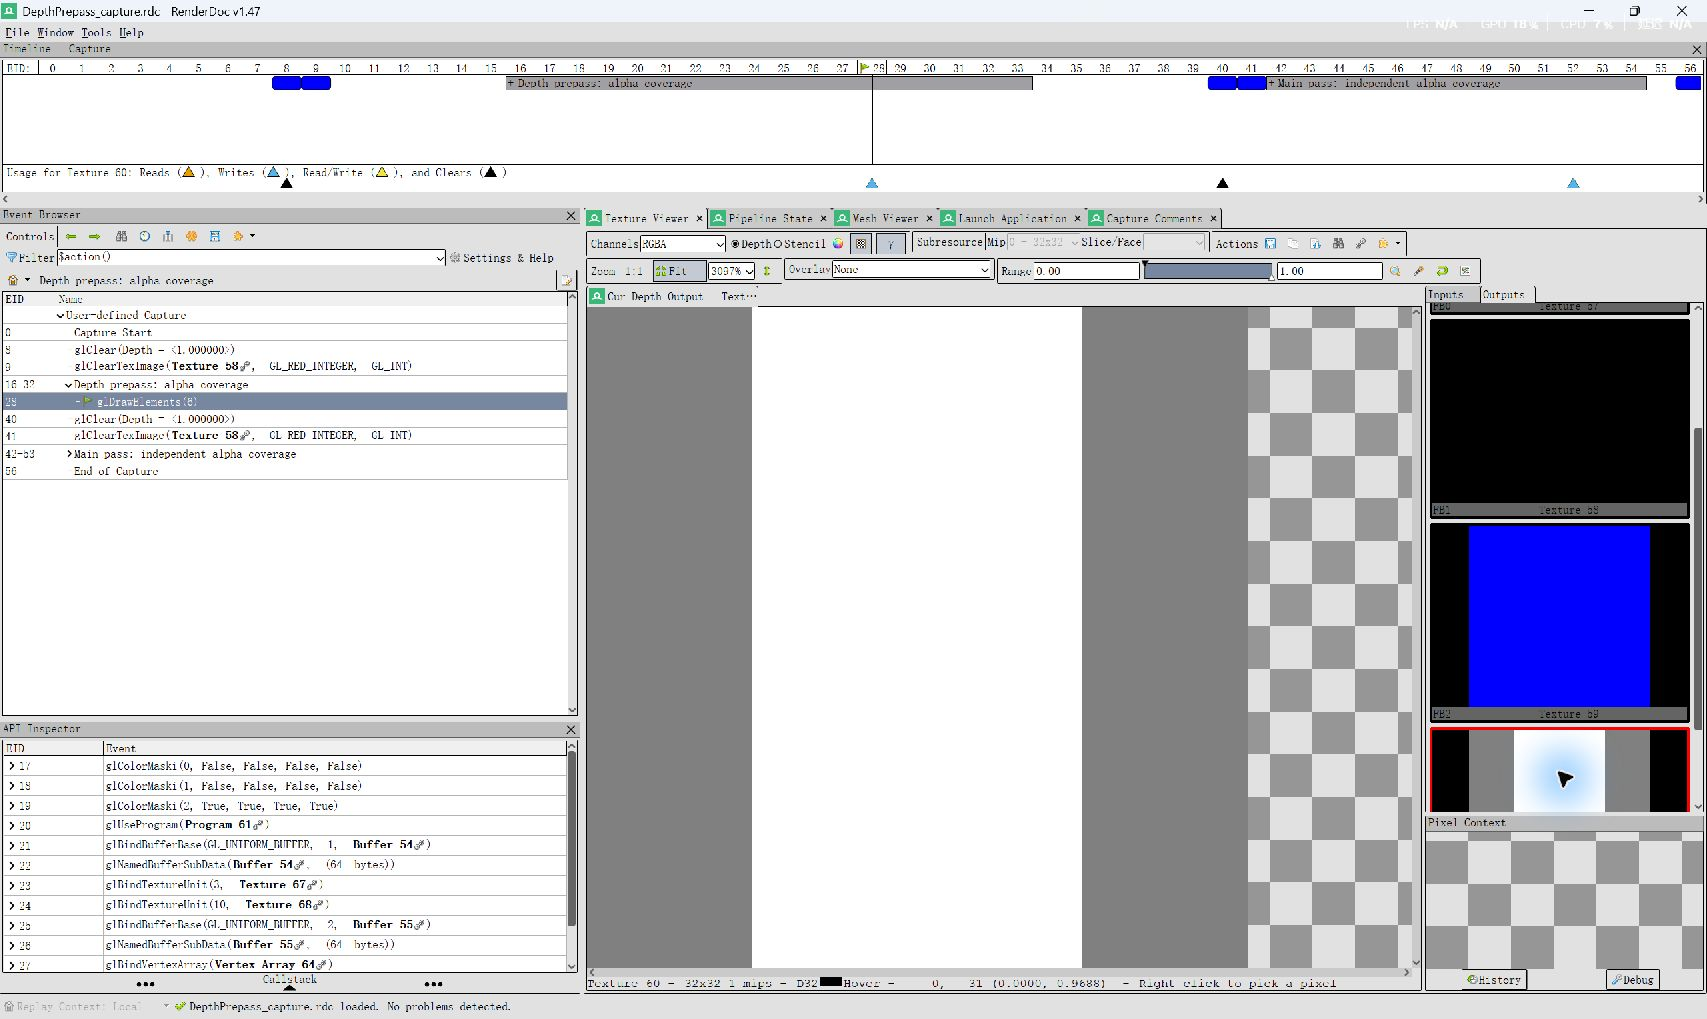
\includegraphics[width=.89\linewidth]{../../../output/captures/renderdoc-eid28-depth.jpg}
\caption{RenderDoc 1.47 回放窗口。事件 28 显示第一次绘制写入的深度图。沿左侧列表往下是清屏和主绘制，可切到事件 52 比较同一行像素。}
\end{figure}

\subsection{把材质透明度换算成预期像素}
回放显示，两次绘制使用的材质底色 alpha 都是 0.75，底色贴图与透明度贴图都已启用。Mask 阈值是 0.5。中左色带只有底色贴图变透明，中右色带只有透明度图变暗。两种来源单独作用，都应把透明度降到阈值以下。

\noindent\begin{tabularx}{\textwidth}{L{4.1cm}YYYY}
\toprule
输入与结果 & 左 & 中左 & 中右 & 右 \\
\midrule
底色贴图 alpha & 1 & $64/255$ & 1 & 1 \\
透明度贴图红通道 & 1 & 1 & $64/255$ & 1 \\
三项相乘后的 alpha & 0.75 & $\approx0.188$ & $\approx0.188$ & 0.75 \\
像素 & 保留 & 丢弃 & 丢弃 & 保留 \\
\bottomrule
\end{tabularx}

在 $32\times32$ 个像素上，两次绘制的深度逐字节相同。两侧共 512 个像素深度为 0.5，中间 512 个仍是清屏值 1.0。主绘制的实体编号也相应为 42 和 $-1$。这次捕获解释了相机所见的两次裁剪；光源看到的阴影与 RSM 轮廓另有逐像素测试。

在 RTX 5070 Ti Laptop GPU 上使用 RenderDoc 1.33 的 DLL 和 1.6.0 应用接口截帧，再用 1.47 回放。两次绘制各用六个索引。驱动在事件 28 报告顶点着色器因 OpenGL 状态重新编译，记录中没有给出重编译耗时或出现频率。
\note{原始帧、导出的两张深度图和像素读数保存在 \path{output/captures/}。运行 \path{tests/run_depth_tests.cmd} 可复现绘制，截帧参数见 \path{output/captures/README.md}。}

\newpage
\section{CPU 时间线采样}
这份时间线采于后续 3D 复查之前，保留为测量方法与条件的记录，没有为最终代码重新采集性能结果。
本次在 Windows 11、AMD Ryzen 9 8945HX 上运行一个 256×256 离屏用例。64 个 Opaque 四边形共用网格，深度预传递逐个绘制，主绘制走实例化。预热 10 轮后采集 60 轮，没有场景灯光与 IBL，SSAO 和 RSM 分别使用白色与黑色输入，不执行阴影或后处理。项目 Instrumentor 输出了 300 个同线程事件，原始 JSON 导入 Chrome 157.0.8103.79 的 Performance 面板。

\begin{figure}[H]
\centering
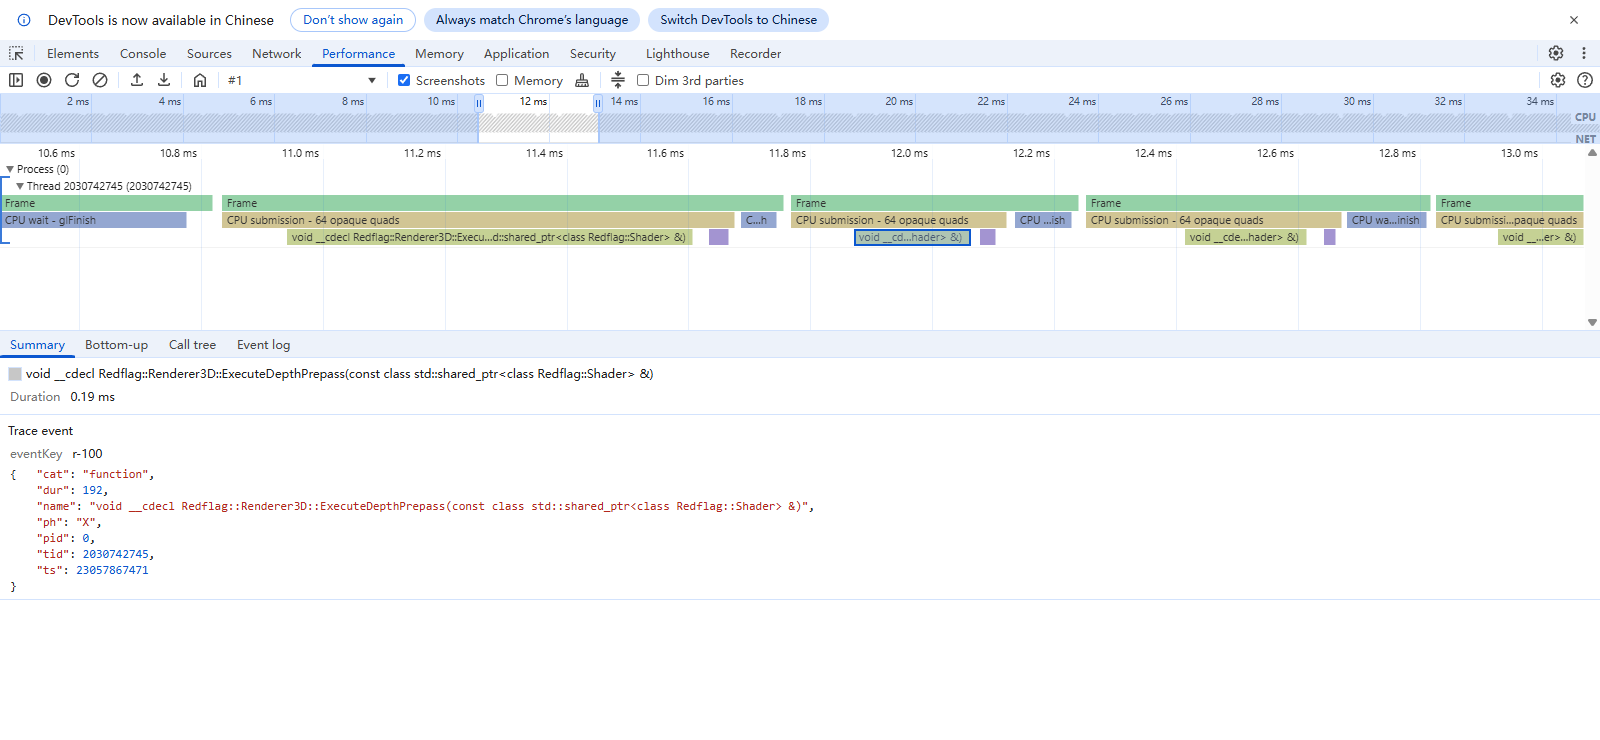
\includegraphics[width=\linewidth]{../../../output/profiling/chrome-cpu-prepass.png}
\caption{Chrome DevTools 实际界面。选中深度预传递的 CPU 区间，原始事件为 192 微秒，界面显示约 0.19 毫秒}
\end{figure}

\begin{tabularx}{\textwidth}{L{6.2cm}Y}
\toprule
CPU 区间 & 60 轮中位数（微秒） \\
\midrule
提交 64 个四边形及两次渲染阶段 & 347 \\
其中：深度预传递 & 199 \\
其中：主绘制 EndScene & 19.5 \\
glFinish 等待 & 66.5 \\
一轮采样 Frame & 467 \\
\bottomrule
\end{tabularx}

这些区间有嵌套关系，不能相加。截图同一轮的 glFinish 等待为 94 微秒，另一张实际截图保存在同目录。它表示 CPU 等待 GPU 完成的时间，不是 GPU 自身执行某个 Pass 的时间。

本次使用 Debug 配置，逐事件写日志并 flush 会干扰采样。每轮 glFinish 又人为串行化了 CPU 与 GPU，没有交换窗口缓冲或完整编辑器工作负载。这里没有优化前后对照，Frame 的倒数不能当作编辑器帧率。后续需要在代表性场景中减少测量干扰并单独获取 GPU 计时。Chrome 的网页专属指标不适用于这份 C++ 时间线。

\note{复现：\path{tests/run_profile_tests.cmd}。原始数据：\path{output/profiling/redflag-cpu-trace.json}，39599 字节；截图和采集说明位于同目录。参考：\source{https://developer.chrome.com/docs/devtools/performance/reference}{Chrome DevTools Performance 功能文档}。}


\newpage
\section{画面近似与下一轮性能比较}
\subsection{保留亮部和反射的代价}
从 HDR 环境图计算光照时，Redflag 将输入中有限的亮度值限制到 $[0,50]$。例如一个值为 100 的亮点会按 50 参与计算，能压低极亮点带来的干扰，也会减少它对环境照明的贡献。光晕在几张不同大小的图上累加，合成时又限制加回场景的亮度。两项处理都改变了能量，比较效果时需要保留同一曝光和输入贴图。
\loc{Redflag/src/Redflag/Renderer/IBLPrecompute.cpp}

RSM 用方向光看到的表面估算一次漫反射。Redflag 让采样点覆盖固定半径的圆盘，修正了光源投影面积与两端漫反射系数。减少采样数仍然覆盖同一范围，取样更稀，画面可能变得更嘈杂。圆盘外的贡献未计入，两点之间也没有再追一条光线查遮挡，近距离还有限制项。因此，同一块白地板上出现了红墙的反光，只能检验反射方向和颜色，还需要单独测噪声和开销。

配套的《渲染公式与实现》给出圆盘、面积与着色器的推导。\path{tests/run_rsm_scene_tests.ps1} 固定相机和灯光，比较开启与关闭 RSM 时同一世界位置的线性颜色差值。用这种方式才能区别真实的红色反射与显示曝光改变造成的颜色变化。
\loc{Redflag/src/Redflag/Renderer/SceneRenderer.cpp}

\subsection{给同一场景做两次可比的测量}
下一轮可先选定 Cornell Box 的相机、灯光、分辨率和曝光，固定驱动、构建方式和功能开关，只改一个要比较的选项。比如比较 RSM 采样数时，预热两组到相同帧数，然后重复记录 CPU 提交时间、GPU 执行时间和同一地板区域的颜色波动。这样才能回答，少采一些点节省了多少时间，又失去了多少稳定性。

比较实例化时还要保持模型数量和屏幕覆盖范围相同，记录分组数与实际绘制次数。比较深度预览时按相同尺寸分别开关面板；比较着色器缓存时把磁盘冷缓存和命中缓存分开。分别保存采样次数、中位数和波动范围，再回头用 RenderDoc 查看异常帧用了哪些资源。上一页的 Chrome 数据回答了 CPU 在哪个区间花时间；完整场景的 GPU 性能还要靠这样的对照实验来测。

引擎分层可对照 Jason Gregory《游戏引擎架构》和 GAMES104。要复习光照、采样及实时近似，再看 GAMES101、GAMES202。本项目引用的版次、章节与原始入口收在 \path{docs/Graphics-References.md}。
\clearpage
\section{网格与材质的着色器接口}
有十把摆在不同位置的椅子，木纹来自同一张贴图。一个物体单独绘制时，CPU 交给着色器一份模型矩阵和一个实体编号；合在一次绘制里时，GPU 要能为每把椅子分别读到这两样东西。无论在哪个位置，木纹该有多粗糙、哪一侧能看见高光，都可以用同一段材质代码计算。

这个约定称为着色器接口。顶点阶段读取网格的位置、法线、纹理坐标和切线；片元阶段读取材质的底色、粗糙度以及相机和灯的位置。Redflag 把共用的光照代码放在一个网格着色器文件里，创建程序时按用途选择不同的输入或输出。发行版里的每个程序只包含它所选的那种画法。

\noindent\begin{tabularx}{\textwidth}{L{3.15cm}YY}
\toprule
OpenGL 画法 & 每个物体提供什么 & 绘制后留下什么 \\\midrule
普通模型 & 当前物体的模型矩阵、材质和编号 & 不透明表面的颜色和编号 \\
\code{INSTANCED} & 每个实例各自的位置、颜色、材质数值和编号 & 同一张画面上仍能选中不同的椅子 \\
\code{TRANSPARENT} & 透明度、折射率和厚度，以及普通网格用的材质数据 & 玻璃颜色、朝向和透光数据，等背景画完再合成 \\\bottomrule
\end{tabularx}

以玻璃为例，背景只画一次。每片玻璃让多少背景光通过，取决于材质的透明度；两片各透过一半的玻璃叠起来，背景光剩四分之一。后端把每片的透光率取对数后相加，最后用下面这段恢复乘积。这样交换两片玻璃的提交顺序也能得到同一个透光率。几层玻璃的表面颜色采用加权平均，颜色与真实的多层光学过程仍有差别。

\begin{verbatim}
// optics.x 存各层透光率的对数之和，取 exp 得到总透光率。
float transmittance = exp(optics.x);
// 按总透光率混合玻璃的平均颜色和它后面的场景颜色。
o_Color = vec4(mix(sum.rgb / sum.a, background, transmittance), 1.0);
\end{verbatim}
\loc{RedflagForge/assets/shaders/Transparency_Composite.glsl}
这两行位于全屏合成的片元 \code{main}。三种网格画法的创建入口在 \path{Redflag/src/Redflag/Renderer/Renderer3D.cpp}，共用材质见 \path{RedflagForge/assets/shaders/Renderer3D_Mesh.glsl}。加权透明的原理可读 \source{https://jcgt.org/published/0002/02/09/}{McGuire 与 Bavoil，Weighted Blended Order-Independent Transparency}。
\clearpage
\section{远处铁丝的取样}
近看一根铁丝，它能占好几个像素，每个像素大致可以判断为铁丝或背景。镜头拉远后，一个像素可能同时盖住铁丝和后面的墙。要比较两种画法，可以先算铁丝在每个像素内实际占了多大面积。若铁丝挡住四分之一，这个像素的颜色也应保留后面四分之三的墙面。

\begin{figure}[H]\centering
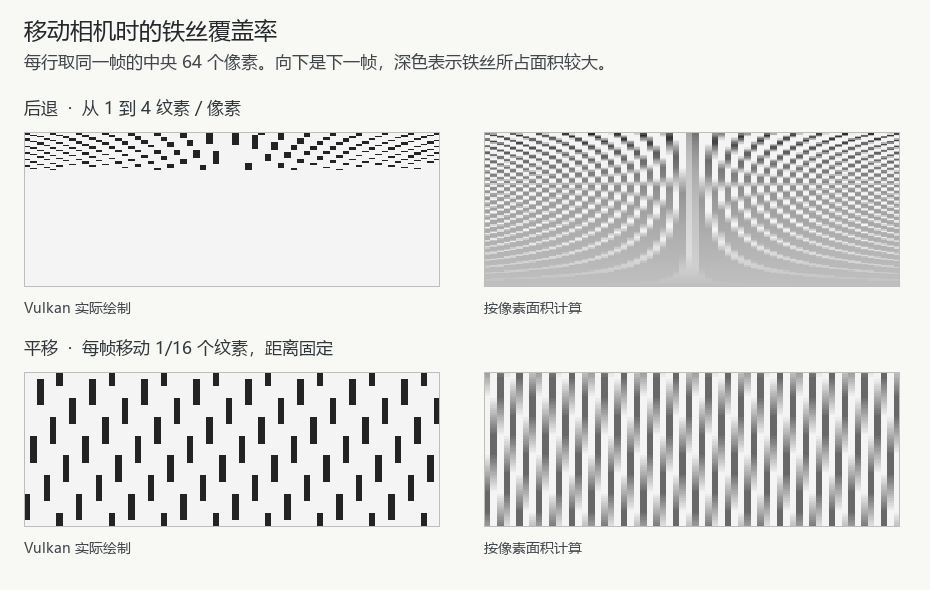
\includegraphics[width=.82\linewidth]{../../../output/validation/fine-mask-motion/motion.png}
\caption{左列是加入 SSAA 前的 Vulkan 单点绘制，右列按同一相机位置计算面积。每一行是该帧画面中央的一排像素，向下读就是镜头的运动过程。后退时左上图变成整片浅色，说明渲染丢掉了铁丝。测试所用引擎库的 SHA-256 以 \texttt{36d47099} 开头。}
\end{figure}

相机不动时，连续 8 帧逐像素相同。让相机每帧横移相当于原图十六分之一列的距离，铁丝在画面中仍应平均占 25\% 的面积。正式绘制却在 12.5\% 和 25\% 之间跳了 16 次。其中相邻两帧有 512 个像素一起从空隙变为铁丝。在另一次缓慢后退的测试里，从一个屏幕像素横跨 1.75 个纹素起，铁丝连续 91 帧消失。拾取轮廓与绘制轮廓始终一致，问题出在两者共用的材质裁剪。\href{run:../validation/fine-mask-motion/report.json}{195 帧的实测}\quad\href{run:../validation/fine-mask-motion/frames.csv}{逐帧数据}

我们试算了另一种选择。在每个像素覆盖的区域内固定选一个点，读取原图的透明度。这样铁丝不会在缩图时被抹掉。在一个像素横跨 26.51 个纹素的固定机位上，这个办法让铁丝占到 25.83\%，接近面积参考的 24.98\%。但放大单个像素看，它仍然只有完全遮挡和完全透光两种结果。整块网的面积接近了，画面里却多出了黑白颗粒。\href{run:../validation/fine-mask/coverage-candidate.png}{三种取样结果对照}

同一个 CPU 实验把纹理图案横移八分之一个屏幕像素，轮廓和相机保持原位。实际面积在每个像素中平均只变化了约 1.28 个百分点，单点取样却让 35.32\% 的像素直接换色。这个候选保留下来作对照。改用同一帧的多个样本后，仍可沿同一条相机轨迹比较铁丝和墙各占多少，以及相邻帧的颜色变了多少。\href{run:../validation/fine-mask/coverage-candidate.json}{候选计算与取样位置}\quad\href{https://research.nvidia.com/publication/2017-02_hashed-alpha-testing}{Wyman 和 McGuire，I3D 2017}

\clearpage
\subsection{一个像素里的两种表面}
铁丝前面有灯，后面是一堵暗墙。放大两者交界的一个像素，其中四分之一是铁丝，余下的部分透过网孔看见墙。假设铁丝着色后红通道的线性值为 $4.0$，墙为 $0.2$。线性值与收到的光量成正比，这个像素的红色应当是多少？

\begin{figure}[H]\centering
\begin{tikzpicture}[font=\small,x=1cm,y=1cm]
\definecolor{samplewall}{HTML}{DEF1F1}
\definecolor{samplewire}{HTML}{F4CAA0}
\begin{scope}
  \fill[samplewall] (0,0) rectangle (2.5,2.5);
  \fill[samplewire] (0,2.5) -- (0,1.25) -- (2.5,2.5) -- cycle;
  \draw[line] (0,1.25) -- (2.5,1.25) (1.25,0) -- (1.25,2.5);
  \draw[ink] (0,0) rectangle (2.5,2.5);
  \foreach \x/\y in {.625/.625,.625/1.875,1.875/.625,1.875/1.875}
    \fill[ink] (\x,\y) circle (2.4pt);
\end{scope}
\node[align=left,anchor=west,text width=9.5cm] at (3.0,1.25) {\textbf{把一个像素放大看}\\[4pt]
橙色是铁丝的边缘，浅蓝色是后面的墙。四个点各代表同样大的取样区域。一个点看见铁丝，另外三个点分别看见墙。};
\end{tikzpicture}
\caption{项目绘制的面积示意。图中铁丝占据像素四分之一的面积，四点估计碰巧与它相等。铁丝再偏一点，四个点数出的比例可能与实际面积有差别。}
\end{figure}

把屏幕上的这个像素均分为四份，各画一次深度和材质，灯光就能照到各自可见的表面。最后将四份的颜色相加，再除以四。图中的红通道得到
\[
  L_{\mathrm{red}}=\frac{4.0+0.2+0.2+0.2}{4}=1.15.
\]
绿色和蓝色也这样计算。场景面板用 $0$ 到 $1$ 表示从黑到白，计算光照的图像却需要保留 $4.0$ 这个亮度。若先把四个数各自截到 $1$，再平均，就只得到 $0.4$。Redflag 把亮部压到可显示范围的处理称为色调映射，安排在颜色平均之后。像素覆盖面积与滤波权重的推导见 \source{https://www.pbr-book.org/4ed/Sampling_and_Reconstruction/Image_Reconstruction}{PBRT 第四版，§8.8}。

Redflag 的延迟渲染先为每个取样位置保存可见表面，再计算光照。\path{Redflag/src/Platform/Vulkan/Shaders/Mesh.frag} 将底色、粗糙度和法线写入场景图，同目录的 \path{PackSurfaces.comp} 用该点的深度还原空间位置。把铁丝和墙的深度先平均，会把光照位置放到两者之间的空处。取样位置各自通过深度测试，光照算完后才有四个可以相加的颜色。Intel 在 SIGGRAPH 2010 的课程里把样本分开处理。普通表面只算一次光照，在同一像素出现不同表面的边缘才逐样本着色。这是今后可以用来比较开销的一种办法。\source{https://www.intel.com/content/www/us/en/developer/articles/technical/deferred-rendering-for-current-and-future-rendering-pipelines.html}{Lauritzen，Deferred Rendering for Current and Future Rendering Pipelines}

Vulkan 编辑器开启 \code{SSAA 2×2} 后，\path{RedflagForge/src/LightingPreview.cpp} 的 \code{Render} 把光照图的宽和高各扩大一倍。几何、着色、屏幕效果仍按原来的顺序执行，内部光照图现在有四倍的像素要算。最终面板保持原来的像素数。下段是面板显示着色器的简化写法，\code{nextRow} 是放大后的图宽。拾取单独绘制一张实体编号图，沿用原来的相机和裁剪，不会对四个物体编号取平均。

\begin{verbatim}
// 伪代码，i 对应每组四个位置的第一项。颜色按行存放。
red = (light[i].r         + light[i + 1].r
     + light[i + nextRow].r + light[i + nextRow + 1].r) / 4;
// 亮度先压到可显示范围，再换成面板所用的显示值。
panelRed = pow(red / (1 + red), 1.0 / 2.2);
\end{verbatim}
\loc{RedflagForge/src/Shaders/LightingPreview.comp}

\clearpage
\subsection{一张黑白铁丝图缩小以后}
试验原图的每四列有一列白色铁丝，另外三列为黑色网孔。四列缩到一个纹素，就留下约 $0.25$ 的灰色。若照近处的方式把这个值与 $0.5$ 比较，四个取样位置都会落到网孔。单靠把光照图画大，仍然可能整片漏掉远处的网。Yüksel 在 I3D 2018 的文章里展示了胡须随镜头拉远而变稀的对照图，作者的方法在预处理缩小贴图时重新分配透明度。Redflag 保留原贴图，在绘制时决定每个样本是否通过。\source{https://www.cemyuksel.com/research/alphadistribution/}{Yüksel，Alpha Distribution for Alpha Testing}

\begin{figure}[H]\centering
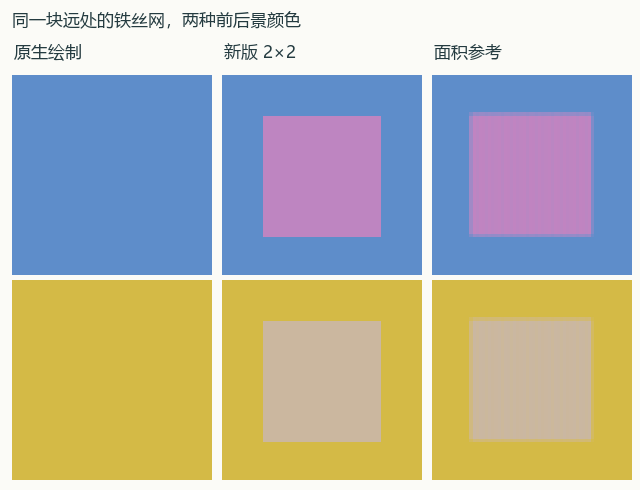
\includegraphics[width=.58\linewidth]{../../../output/validation/mask-supersampling-current/two-colors.png}
\caption{同一个网格，两组自发光材质。每个面板像素横跨原图 26.5 列。左列是单点绘制，看不见铁丝。中列是四点绘制，能看到前后景混出的颜色。右列用每个像素里实心部分的实际宽度计算，网格边缘和内部仍有细微明暗变化。前两列来自 Vulkan 读回，三列使用同一显示转换。}
\end{figure}

在原图上，白色是铁丝，黑色是网孔。镜头拉远时，先读出一个面板像素里四个位置的灰度，再用平均灰度估计铁丝所占的面积。例如四个位置分别读到 $0.95,0.45,0.40,0.20$，平均为 $0.50$，应留下两个位置。先留灰度最大的两处，铁丝的轮廓就能跟着纹理走。四处读数完全相同时才用固定顺序。

每个像素只能留下零到四个样本，能表示的面积比例相隔四分之一。因此四个通过值选在每两档的中间，即 $1/8,3/8,5/8,7/8$。平均灰度为 $0.25$ 时只过第一档，留下的那个样本看见铁丝，其余三个看见墙。近处仍按每处自己的灰度与 $0.5$ 比较。屏幕像素从覆盖一个原图纹素逐渐变成覆盖两个纹素时，着色器逐渐转用四处平均和排序。正式代码在 \path{Shaders/Cutout.glsl} 的 \code{coversArea}。

这条规则只用于一种可以从贴图本身确认的材质。底色图的透明度或独立透明图的红通道，须有一张只含黑和白，另一张处处为白。设这次绘制传给着色器的透明度系数为 $a>0$，材质的裁剪值还须恰好是 $a/2$。一般灰度图或不同裁剪值仍直接比较完整的透明度。若两张纹理都决定网孔的位置，单看各自的平均数会弄错图形。比如一张只让左半边通过，另一张只让右半边通过，两张相乘后处处为黑，而两个平均值相乘却是 $0.25$。实际条件见 \path{Redflag/src/Platform/Vulkan/VulkanDraw.cpp} 的 \code{DrawIndexed}，透明度比较在同目录的 \path{Shaders/Cutout.glsl}。

两张网在同一个像素内重叠时，缩图还会丢掉前后两层的相对位置。把两张网叠放，每张各挡四分之一；将后面那张的花纹平移两列，真实的两组铁丝合计遮住一半。缩小后，两张图都给出 $0.25$，于是两层网挑中同一个取样位置。这次 GPU 实测只留下四分之一的铁丝。深度测试仍能选对每个位置前面的那层，没保留下来的是两层铁丝在像素中原本错开的距离。\href{run:../validation/mask-supersampling/subpixel-materials.csv}{单层与两层网的 Vulkan 读回}

Vulkan 也提供由透明度决定多个样本是否保留的功能（alpha-to-coverage），规范读取的是第一个颜色输出中的 alpha。Redflag 的这一个值存着粗糙度和金属度，还用符号区分发光表面。为保留现有材质数据，编辑器直接在放大的光照图上取样。\source{https://docs.vulkan.org/spec/latest/chapters/fragops.html\#fragops-covg}{Khronos，Fragment Operations，Multisample Coverage}

\clearpage
\subsection{移动镜头时的铁丝颜色}
铁丝和背板分别用固定的颜色发光。假设某一帧、某个像素里铁丝占比为 $p$，用铁丝颜色乘以 $p$，再加上墙的颜色乘以 $1-p$，就得到该像素的参照颜色。$p$ 可以直接由镜头位置和铁丝在原图中的宽度算出。测试将两组前后景颜色交换明暗并改变色相，分别用 Vulkan 绘制，再读取 $64\times64$ 幅面的线性 RGB。图中每列除了最右侧的数学参照，都是 GPU 的结果。

\begin{figure}[H]\centering
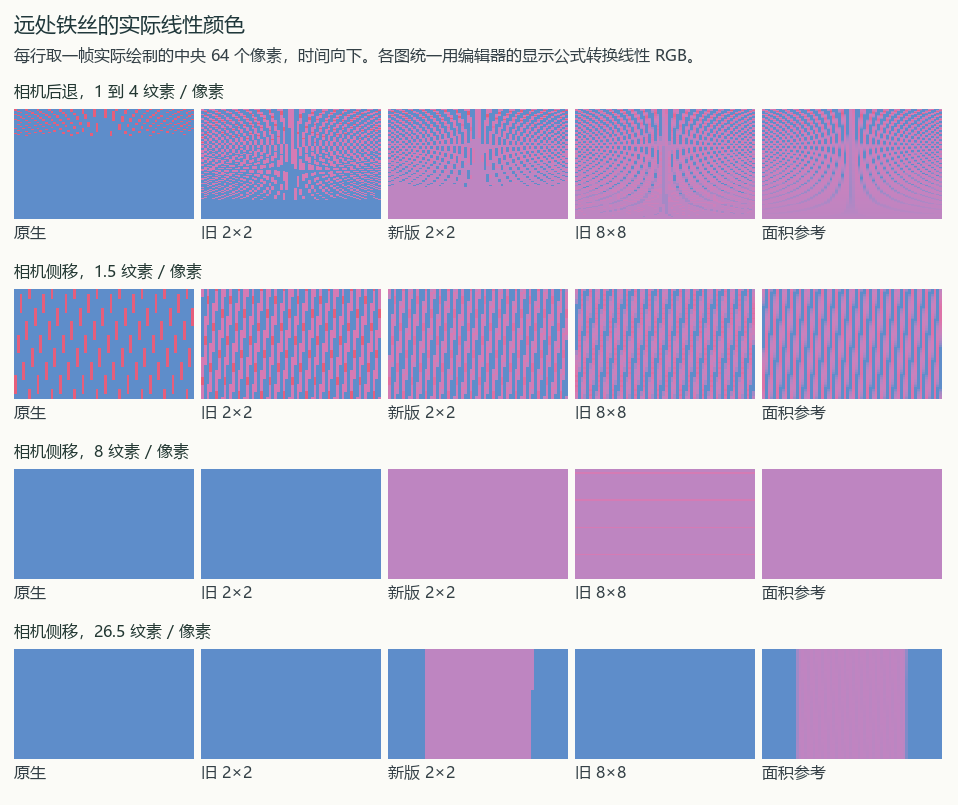
\includegraphics[width=.94\linewidth,trim=0 373bp 0 0,clip]{../../../output/validation/mask-supersampling-current/motion.png}
\caption{每幅图里，时间都从上往下读。上排让相机缓慢后退，下排让相机水平移动。图中的“旧 $2\times2$”和“旧 $8\times8$”仅提高分辨率，每个位置仍一律按 $0.5$ 裁剪。对照最右侧的实际面积，上排第一幅有大片帧只剩蓝底，第三幅还能看见铁丝。\href{run:../validation/mask-supersampling-current/motion.png}{查看含两组远景的完整实测图}}
\end{figure}

比较闪动，要扣除相机真的移动所产生的变化。比如原图预测某一像素的铁丝从占 20\% 变为 22\%，绘制却从完全空变成四分之一实心，那么这次绘制多跳了 $25-2=23$ 个百分点。把这种差的绝对值对每个像素、每对相邻帧取平均，得到“变化误差”。另一个指标“覆盖误差”直接比较每个像素里画出的比例与实际面积。这两项分别回答画面跳了多少、铁丝占得准不准。\href{run:../validation/mask-supersampling-current/frames.csv}{各帧机位和误差}\quad\href{run:../validation/mask-supersampling-current/report.json}{设备、程序与 GPU 读回}

{\small\noindent\begin{tabularx}{\linewidth}{@{}Yrrr@{}}\toprule
竖铁丝，误差单位为百分点 & 单点 & 初版四点 & 四点按灰度排序 \\\midrule
镜头后退，覆盖误差 & 23.29 & 8.56 & 5.44 \\
镜头后退，变化误差 & 9.90 & 10.59 & 5.54 \\
镜头平移，覆盖误差 & 20.06 & 9.13 & 5.32 \\
镜头平移，变化误差 & 5.08 & 4.95 & 3.91 \\\bottomrule
\end{tabularx}\par}

后退的 121 帧里，单点绘制末尾连续 91 帧只剩背景。表中的“初版四点”给四个位置各分配一个固定的通过值，保住了网，变化误差却比单点还高。让四个位置共用面积估计，再优先留下最接近铁丝的位置，两项误差都降低了。改用斜铁丝，后退时变化误差也从初版四点的 9.24 降到 6.01 个百分点。每像素横跨 26.5 个纹素的远景里，中央区域保有四分之一的铁丝，网格外沿仍能看出四点取样与实际面积的差距。\href{run:../validation/mask-footprint-compare-rank/report.json}{不同方向的逐项实测}

在仓库根目录运行 \path{tests/run_mask_supersampling.cmd} 可重画竖铁丝。\path{tests/MaskSupersampling.cpp} 的 \code{Measure} 为两张自发光方片分别写深度和颜色，再执行显示着色器。测量用 Debug x64 和 RTX 5070 Ti Laptop GPU。对 Sponza 的 $384\times246$ 输出，逐帧着色的位置会从 94,464 增到 377,856。因此编辑器默认关闭 SSAA。整帧时间、显存和 RenderDoc 回放见《渲染性能实测》的“SSAA 的四个着色样点”。\href{run:Redflag-Rendering-Performance.pdf}{渲染性能实测}

\end{document}
